\begin{figure}
\centering
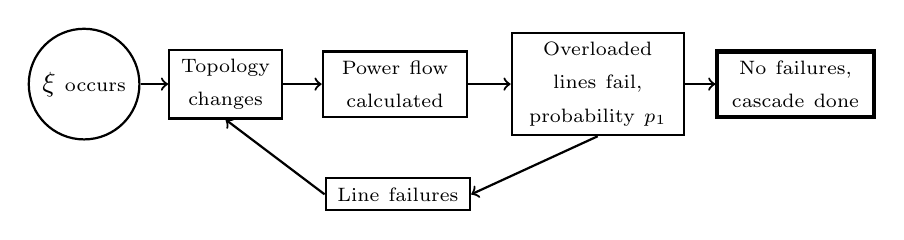
\begin{tikzpicture}
\draw [->,thick] (1,1) node[anchor=east, circle, draw]{$\xi$ \scriptsize occurs}
-- (1.35,1) node(TC)[anchor=west,text width=1.2cm,text centered,  rectangle, draw]{\scriptsize Topology changes};
\draw[->,thick] (TC)
--(3.3,1) node(PF)[anchor=west,text width=1.6cm,text centered, rectangle,draw]{\scriptsize Power flow calculated};
\draw[->,thick] (PF)
--(5.7,1) node(F)[anchor=west,text width=1.95cm, text centered, rectangle, draw]{\scriptsize Overloaded lines fail, probability $p_1$};
\draw[->,thick] (F)
--(8.3,1) node(DN)[anchor=west,text width=1.75cm, text centered,rectangle,draw,line width=1.5pt]{\scriptsize No failures, cascade done};
\draw[->,thick] (F.south)
--(5.2,-.4) node(LF)[anchor=east,text width=1.6cm, text centered, rectangle, draw]{\scriptsize Line failures };
\draw[->,thick] (LF.west)
-- (TC.south);

\end{tikzpicture} 
\caption{OPA simulation of a cascading power failure}
  \label{fig:cascade}
\end{figure}
